\section{Experiments}
\label{sec:experiments}

\subsection{The influence of synthesized segmention noises on feature transferability}
\label{subsec:robustness}

%%%%%%%% TEXT Experiment setup

\paragraph{Experiment setup}
To investigate the influence of inexhaustive segmentations, misclassifications and false segmentations on feature transferability, we set up experiments with synthesized label noises from a well-annotated dataset, the PASCAL VOC2011 segmentaion dataset\cite{everingham2015pascal}.
Fifteen out of twenty categories of the VOC2011 dataset were selected to form a \textit{pre-training dataset} and the other categories formed a \textit{fine-tuning dataset}.
The pre-training dataset was used to train a Fully Convolutional Network with AlexNet (FCN-AlexNet) model\cite{long2015fully} for segmentation in the precense or absence of synthesized segmentation errors.
The fine-tuning dataset was used to fine-tune the weights of convolutional layers from the pre-trained FCN-AlexNet models.
Inexhaustive segmentations, misclassifications and false segmentations were synthesized separately with stochastical corruptions to the well-annotated pre-training dataset, followed the descriptions in Section \ref{subsec:formulation}.
Fine-tuned models were evaluated by mean intersection over union ratio (mean IU) achieved on the fine-tuning test set, referring to as the \textit{fine-tuning performance}.
Performance improvement of fine-tuning transferred models compared to an randomly initialized model indicates the transferability of pre-trained weights.

\paragraph{Experiment details}
To avoid that the choice of pre-training and fine-tuning splitting for categories influence the results, the 20 categories of VOC2011 were divided equally into four folds.
Each fold was studied separately, and the exact partitions of each fold is listed in Table \ref{tab:robustness}.
The training dataset was enriched with extra segmentations by Hariharan et al.\cite{hariharan2011semantic}
To keep the segmentation task simple, we used only single-object images, resulting in totally 4000 training images for 20 categories available for pre-training, fine-tuning dataset and evaluation.
In order to accelerate the training process, we subsampled the original images by four times.
Fully Convolutional Networks with AlexNet was used for experiments because its relatively small capacity and thus short training time.
The existence of an ImageNet model for AlexNet can be beneficial to set a performance reference.
The non-transferred layers were random initialized with Xavier Initialization.
The ImageNet model and completely random weight initialization were considered as the upper bound and lower bound, respectively, for various pre-trained weights summarized in Table \ref{tab:robustness}.
The default hyperparameters of FCN-AlexNet in \cite{long2015fully} were kept unchanged.
Training run 240,000 iterations for pre-training phase, and 12,000 iterations for fine-tuning phase.
Snapshots for trained models were taken every 4,000 iterations.
Each experiment was repeated three times, mean and standard deviation were computed over the last five snapshots for all repetitions.


% \noindent \textit{What Table \ref{tab:robustness} tell us.
% How annotation errors were synthesized;
% How synthesizations are different from reality;
% Transferability of noisy models compared to clean models.
% }


\paragraph{Inexaustive Segmentation}
Fine-tuning performances of transferring models pre-trained with complete labels and half of the objects unsegmented respectively are summarized in Table \ref{tab:robustness}.
The HalfUnsegmented model transferred into a fine-tuned model with an average mean IU 0.04 worse than the CompleteLabels model, almost the same as training a model with random weight initialization.
This result indicates that inexhaustive segmentation can have negative impact on weights transferability.
By applying the sigmoidal negative loss to pre-train models with half of the objects segmented, we were able to achieve a comparable fine-tuning performance as using the complete segmentation to pre-train.
The details of implementing sigmoidal negative loss for the pre-training dataset will be discussed in Section \ref{subsec:pulearning}.

\paragraph{Misclassifications}
Models pre-trained with random labels are listed in Table \ref{tab:robustness}.
% The noisy dataset containing labels for target segments stochastically transited to a random class with probability $p_{jk}=\frac{1}{20}$.
% The resulted trained model was denoted as the AllRandomLabels model in Table \ref{tab:robustness}.
% Similiarly, if a random half of the segmented objects were assigned random labels, the resulting pre-trained model is called the HalfRandomLabels model.
% The noise-free counterpart of these two noisy models was the model trained with true labels, denoting as the TrueLabels model.
% True labels can be considered as labels transiting with probability $p_{jk}=\delta(j-k)$.
% $$p(\tilde{y_{ij}}=l \vert y_{ij}=k) = \delta(l-k)$$.
Compared to the CompleteLabels model (the one trained with true labels), both the model trained with all random labels or half true half random labels led to worse fine-tuning performances.
Fine-tuned performances of the AllRandomLabels model and the HalfRandomLabels model were no better than randomly initializing model weights, indicating poor weights transferabilities of a trained model in the presence of random labels to segmentations.
In other words, misclassification noises in segmentation can impact the transferability of convolutional weights negatively.

However, binarizing labels for pre-training was able to achieve equivalent fine-tuning performance as using true labels.
It achieved better performance than training to segment the exact classes but with random labels.
Binarized labels are accurate but imprecise because pixel labels were randomized among foreground classes and binarizing labels lead to correct segmention for foreground and background.
This observation indicates that inaccurate labels may have more significant negative influence than imprecise labels for feature transferability.

% The small pre-training dataset can be a reason of similarly performed binary and multi-class pre-trained models.
% In our experiment, most classes had only around one hundred images, and the dining table had only 20 images.
% The limited number of class samples may increase the difficulty to segment individual classes and may explain why binarized labels could achieve comparable fine-tuning performance to true labels.

Additionaly, we studied the influence of categorizing classes for pre-training to keep the labels precise to some extent.
We categorized the fifteen classes in the pre-training set into person, animal, vehicle, indoor according to \cite{everingham2015pascal} and trained a model to transfer, shown as the error bars on lines in figure \ref{fig:categories} at categories 4.
As a comparison, the fifteen classes were also randomly categorized into 4, 7, 11 categories and shown as isolated error bars in figure \ref{fig:categories} at categories 4, 7, 11 respectively.
Figure \ref{fig:categories} shows that categorizing pre-training classes had little effect to the fine-tuning performance of transferred models.
Even categorizing classes at random without explicit meaning could pre-train weights better than random initialization (shown as error bar at categories 0).
It can be beneficial to binarize or group classes into hyper-categories to learn better transferable weights in the presence of misclassifications.

\paragraph{False segmentations}
To synthesize mis-segmentation noises, we selected one category, either cat or dog depending on the folds, as the target category and all the other 14 categories in the pre-training dataset became non-target, as discussed in Section \ref{subsec:formulation}.
In the presence of mis-segmentation noises, instances from non-target categories can be misannotated as the target category with probability of $p_{1} = 1$ and $p_{1}= 0.5$ respectively.
The two choices of probability led to two different pre-training sets and thus two different pre-trained models, naming the AllMisSegmented model and the HalfMisSegmented model, in Table \ref{tab:robustness} respectively.
The noise-free counterpart of mis-segmentation is an dataset containing segmentations of the selected target category only whilt the other 14 categories remained unsegmented.
Model trained with this noise-free dataset was denoted as NoMisSegmented in Table \ref{tab:robustness}.

\noindent
Table \ref{tab:robustness} shows that all three models achieved better fine-tuning performances than random initialization.
The dataset mis-segmented all non-target instances produced a model with even slightly better fine-tuning performance than the dataset segmented only the target category.
However, it is less likely to happen in practice that annotators will mis-segment every single non-target instance in the dataset.
Mis-segmentations often occurr in annotations occasionally.
Therefore, we also trained models with a training set containing half of the non-target objects to test if inexhaustively mis-segmenting non-target objects decreased the fine-tuning performance.
The results show that the HalfMisSegmented model had a slightly worse fine-tuning performance than the AllMisSegmented model but was still comparable to the NoMisSegmented model.
Based on these observations, we concluded that mis-segmenting semantically meaningful objects could have little impact when they are used for pre-training transferable weights.



\begin{table*}[t]
\resizebox{\textwidth}{!}{
\centering
\begin{tabular}{l|l|llll|l}

\hline
                                                                                      & \begin{tabular}[c]{@{}c@{}}Initial Feature\\ Extractor\end{tabular} & \multicolumn{4}{c|}{Fine-tuning mean IU per pretraining-finetuning fold}                                                                                                                                                                                                                                                                                                                                                                     & \multicolumn{1}{l}{\multirow{2}{*}{\begin{tabular}[c]{@{}l@{}}Average \\ mean IU\\ across \\ four folds\end{tabular}}} \\ \cline{1-6}
\begin{tabular}[c]{@{}l@{}}Fine-tuning\\ categories\end{tabular}                      &                                                                     & \multicolumn{1}{l}{\begin{tabular}[c]{@{}l@{}}aeroplane, \\ bicycle, bird,\\ boat, bottle\end{tabular}} & \multicolumn{1}{l}{\begin{tabular}[c]{@{}l@{}}bus, car, \\ cat, \\ chair, cow\end{tabular}} & \multicolumn{1}{l}{\begin{tabular}[c]{@{}l@{}}dining table,\\ dog, horse, \\ motorbike,\\ person\end{tabular}} & \multicolumn{1}{l|}{\begin{tabular}[c]{@{}l@{}}potted plant, \\ sheep, sofa, \\ train, TV\end{tabular}} & \multicolumn{1}{l}{}                                                                                                   \\ \hline
\multirow{2}{*}{\begin{tabular}[c]{@{}l@{}}Upper bound \&\\ lower bound\end{tabular}} & ImageNetModel                                                       & $0.42\pm0.01$                                                                                           & $0.51\pm0.01$                                                                               & $0.49\pm0.01$                                                                                                  & $0.47\pm0.01$                                                                                           & $0.47\pm0.01$                                                                                                          \\
                                                                                      & RandomWeights                                                       & $0.29\pm0.01$                                                                                           & $0.29\pm0.03$                                                                               & $0.27\pm0.01$                                                                                                  & $0.30\pm0.02$                                                                                           & $0.29\pm0.02$                                                                                                          \\ \hline
\multirow{3}{*}{\begin{tabular}[c]{@{}l@{}}Inexaustive \\ Segmention\end{tabular}}    & CompleteLabels                                                      & $0.29\pm0.01$                                                                                           & $0.36\pm0.01$                                                                               & $0.29\pm0.01$                                                                                                  & $0.37\pm0.01$                                                                                           & $\mathbf{0.33\pm0.01}$                                                                                                 \\
                                                                                      & HalfUnsegmented                                                     & $0.26\pm0.01$                                                                                           & $0.30\pm0.03$                                                                               & $0.28\pm0.03$                                                                                                  & $0.32\pm0.02$                                                                                           & $0.29\pm0.02$                                                                                                          \\
                                                                                      & SigmoidalLoss                                                       & \multicolumn{1}{l}{$0.31\pm0.0x$}                                                                       & \multicolumn{1}{l}{$0.37\pm0.0x$}                                                           & \multicolumn{1}{l}{$0.33\pm0.0x$}                                                                              & \multicolumn{1}{l|}{$0.35\pm0.0x$}                                                                      & $\mathbf{0.34\pm0.0x}$                                                                                                 \\ \hline
\multirow{3}{*}{Misclassification}                                                    & AllRandomLabels                                                     & $0.29\pm0.01$                                                                                           & $0.33\pm0.03$                                                                               & $0.26\pm0.01$                                                                                                  & $0.28\pm0.01$                                                                                           & $0.29\pm0.01$                                                                                                          \\
                                                                                      & HalfRandomLabels                                                    & $0.27\pm0.01$                                                                                           & $0.33\pm0.02$                                                                               & $0.25\pm0.01$                                                                                                  & $0.29\pm0.01$                                                                                           & $0.29\pm0.01$                                                                                                          \\
                                                                                      & BinarizedLabels                                                     & $0.30\pm0.02$                                                                                           & $0.35\pm0.01$                                                                               & $0.29\pm0.02$                                                                                                  & $0.35\pm0.03$                                                                                           & $\mathbf{0.32\pm0.02}$                                                                                                 \\ \hline
\multirow{2}{*}{\begin{tabular}[c]{@{}l@{}}False \\ Segmentaion\end{tabular}}         & NoFalseSegmented                                                    & $0.26\pm0.01$                                                                                           & $0.37\pm0.03$                                                                               & $0.27\pm0.01$                                                                                                  & $0.33\pm0.04$                                                                                           & $\mathbf{0.31\pm0.02}$                                                                                                 \\
                                                                                      & FalseSegmentedHalf                                                  & \multicolumn{1}{l}{$0.27\pm0.01$}                                                                       & \multicolumn{1}{l}{$0.34\pm0.01$}                                                           & \multicolumn{1}{l}{$0.30\pm0.01$}                                                                              & \multicolumn{1}{l|}{$0.32\pm0.01$}                                                                      & $\mathbf{0.31\pm0.01}$                                                                                                 \\ \hline

\end{tabular}
}
\caption{Segmentation performance for FCN-AlexNet models pre-trained with 15 categories from the PASCAL VOC2011 dataset and fine-tuned with the other 5 categories.
\textbf{ImageNetModel} represents the pre-trained ImageNet model (upper bound);
\textbf{RandomWeights} indicates that the random initilialized weights (lower bound);
All the other extractors were pre-trained in the presence or absence of the corresponding label noises listed in the leftmost column.
Half of the objects unsegmented result in pre-trained models not significantly better than random weight initialization.
Introducing the sigmoidal negative loss in the pre-training phase was able to improve the fine-tuning performance to be comparable as pretrained model with complete segmentations.
Random labels interefered the fine-tuning performance of transferred models and binarizing classes as foreground and background for in the pre-training dataset help overcome the negative effects of random labels.
Including false segmentions had little influence on transferred models.
% \textit{SingleCategory} was pre-trained on only one annotated category, either ``dog'' or ``cat'' depending on the fold, and the other categories were left unannotated;
% \textit{BinaryLabels} was pre-trained with binary labels that any objects of the fifteen categories were annotated as one single category, namely ``dog'' or ``cat'' depending on fold;
% \textit{TrueLabels} was pre-trained with all objects segmented and assigned to 15 categories correctly;
% \textit{AllRandomLabels} was pre-trained with all objects correctly segmented but assigned random labels;
% \textit{HalfRandomLabels} was pre-trained with all objects correctly segmented and half of them randomly assigned labels;
% \textit{IncompleteLabels} was trained with datasets that objects were annotated correctly with a probability of 0.5;
}
\label{tab:robustness}
\end{table*}


%%%%%%%% Figure categorizing classes
\begin{figure}[t]
\centering
   \includegraphics[width=1.\linewidth]{img/num_classes.eps}
\caption{
Test performance for models fine-tuned from pre-trained weights using data of categorized pre-training classes.
Isolated error bars denote random categorizations (RC) of the 15 classes, while error bars located on lines denote the meaningful categorization.
Zero categorize means no pre-trained weights used and model was random initialized.
The displayed mean IU/mean accuracies and standard deviations were averaged over four folds listed in Table \ref{tab:robustness}.
The trend shows that binarizing and categorizing classes had little negative effect on feature transferability.
}
\label{fig:categories}
\end{figure}


%%%%%%%%%%%%%%%%%%%%%%%%%%%%%%%%%%%%%%%%%%%%%%%%%%%%%%%%%%%%
%%%%%%%%%% PU Learning
%%%%%%%%%%%%%%%%%%%%%%%%%%%%%%%%%%%%%%%%%%%%%%%%%%%%%%%%%%%%

\subsection{Learn to classify with positive and unlabeled samples}
\label{subsec:pulearning}

% In order to compare exponential unlabeled loss with class weighted logistic/softmax loss, we synthesized positive and unlabeled learning setups for classification and segmentation respectively.


\paragraph{2-dimensional moon set}

Figure \ref{fig:moons} shows the decision boundaries of a 2-layer multilayer perceptron, with 6 neurons per layer, trained with the weighted loss, the sigmodal loss and the bootstrapping loss.
Four hundreds samples per class were drawn randomly from two interleaving half circles with noises added with a minor standard deviation.
The leftmost column in the figure shows the multilayer perceptron trained with complete positive labels and the normal logistic loss while the other three columns show the classifier trained with half of the positive examples labeled as negative.
For sigmoidal negative loss, the mis-labeled positive examples farther from the decision boundary have smaller derivatives the ones closer to but still distant from the decision boundary.
As a consiquence, optimization performed as counting the weights update contributions differently for confident and unconfident prediction instead of simply decreasing the overall estimation for the negative loss.
The result decision boundary is more distant from the positve cluster and confident predictions are made in more areas of the space.
% The positive examples push the decision boundary away from the positive cluster while negative examples closed to the decision boundary instead of those away from the decision boundary pull the decision boundary towards the positive cluster.
% The exponential loss was introduced in \cite{tax2016class} to get rid of the effect of outliers.
% In our case, the negative examples given confident predictions by classifier can be considered as outliers.

%%%%%%%% FIGURE MOONS

\begin{figure*}
\begin{center}
% \fbox{\rule{0pt}{2in} \rule{.9\linewidth}{0pt}}
   \includegraphics[width=0.95\linewidth]{img/moons.png}
\end{center}
   \caption{
   Decision boundaries of a 2-layer multilayer perceptron trained with different losses on a 2D moons dataset with unlabeled positive. The \textbf{leftmost} figures have complete positive labels, meaning the positive and negative labels are all correct, whereas, in \textbf{the other figures} only half of the positives were correctly labelled and the rest were mixed with the negative samples. A \textbf{red circle} indicates an example labelled as positive whilst a \textbf{blue square} indicates the example has a negative label. The \textbf{background colors} represent the probability for the area to be positive given by the classifier trained with the given samples and labels: \textbf{red} for high probability areas, \textbf{blue} for low probability areas and \textbf{white} for the class transition areas, i.e.decision boundaries. The \textbf{size of the markers} in the top row denotes the per-class normalized training losses and the \textbf{size of the markers} in the bottom row the per-class normalized derivatives w.r.t the output of the last layer for the trained Multilayer Perceptron (MLP) with the different losses.
   Compared to the normal logistic loss and weighted logistic loss, the sigmoidal negative loss has larger derivatives near the decision boundary. The decision boundary optimized with sigmoidal negative loss is farther away from the positive cluster and thinner.
   }
\label{fig:moons}
\end{figure*}

\paragraph{CIFAR dataset}

In the classification setup, we combined the CIFAR10 dataset and CIFAR100 dataset, using CIFAR10 as the positive (P) set and CIFAR100 as the negative (N) set.
The learning objective is to classify images into eleven classes: ten positive classes from CIFAR10 and a negative class for images from CIFAR100.
Note that there is no category overlap between CIFAR10 dataset and CIFAR100 dataset.
To synthesize a positive and unlabeled (PU) learning setup, we selected only part of positive images from CIFAR10 to be correctly labeled and the rest of the CIFAR10 images were mixed with CIFAR100 images, forming the unlabeled (U) set.
Models were then trained with the labeled part of P set and U set.
An eight layer VGG net was used together with different choices of losses.
The architecture of this VGG8 model can be found in Appendix \ref{sec:support}.
Each model was trained from scratch with Adam optimizer and base learning rate 0.0001.
Model performances were evaluated on a separate test set of combined CIFAR10 and CIFAR100 with true labels.

%%%%%%%% TABLE CIFAR10 50%
Table \ref{tab:cifar} summarizes the test precisions and recalls for training with different losses in the PU setup, compared with training with complete positive labels.
With a training set containing 50\% labeled CIFAR10 images and the rest unlabeled, the normal cross-entropy loss led to an imbalanced model with high precision but low recall, and therefore with a low f1-score.
By reweighing the negative loss by a factor of 0.5, we were able to balance precision and recall and improve the resulting f1-score.
Compared to the negative weighted loss, exponential loss and (hard) bootstrapping loss were able to achieve slightly better f1-scores.
The weighted unlabeled loss and hard bootstrap loss were able to achieve more balanced precision and recall than the exponenetial unlabeled loss.
That is because the two former losses were weighted by classes frequency of observed labels, around 0.67 for the negative class and 2 for positive classes, whereas the exponential unlabeled loss was not.
The reason for this is that reweighing exponential unlabeled loss by observed label frequencies would trade too much precision for recall (0.74 and 0.83 respectively), resulting in a worse f1-score than not reweighing losses.
Compared to the weighted unlabeled loss, the exponential unlabeled loss seems to be more sensible to the choice of class weights and easier over-balancing due to the zero contribution to model updates for confident positive predictions.
One solution to this would be adding a hyperparameter to tune the boundary between confident and unconfident predictions so that a tradeoff between precision and recall can be made in addition to changing the class weights.
Recently, Lin et al. \cite{lin2017focal} proposed a Focal Loss\cite{lin2017focal} for object detection with imbalanced dataset, which takes the form of $l_{y=t} = - \alpha_t (1-p(y=t \vert x)))^{\gamma} \log p(y=t \vert x)$.
This focal loss can be considered as an attempt going towards this direction.


\begin{table}[t]
\resizebox{\columnwidth}{!}{
\centering
\begin{tabular}{ll|llll}
Annotation  & Loss & acc. & mean prec. & mean rec. & mean $F_1$ \\
\hline
Complete    & CrossEntropyU.   & 0.87 & 0.88 & 0.82 & 0.85 \\
50\%(P+N)   & CrossEntropyU.   & 0.83 & 0.84 & 0.78 & 0.80 \\
\hline
50\%P+U     & CrossEntropyU.   & 0.76 & 0.xx & 0.xx & 0.xx \\
50\%P+U     & WeightedU.       & 0.78 & 0.75 & 0.75 & 0.76 \\
50\%P+U     & ExponentialU.    & \textbf{0.81} & \textbf{0.85$\pm0.03$} & 0.72$\pm0.03$ & 0.77 \\
50\%P+U     & BootstrapHard    & 0.80 & 0.76 & \textbf{0.81} & \textbf{0.78} \\
\end{tabular}
}
\caption{Accuracy, mean precision, mean recall and mean f1-score on test set of the CIFAR dataset with true labels.The complete dataset contains images from CIFAR10 as the \textbf{positive} (P) set and images from CIFAR110 as the \textbf{negative} (N) set. The unlabeled positive examples from P set construct the \textbf{unlabeled} (U) set, together with N set. Precision and recall were averaged over ten positive classes. Experiments were repeated three times with random split of P set and U set, and standard deviations were around 0.01 if not explicitly mentioned.}
\label{tab:cifar}
\end{table}


%%%%%%%% FIGURE Varying positive annotating percetage
\noindent
As a reference of the performances, we trained a classifier with 50\% of the positive samples and the same percentage of true negative samples.
We refered this setup as positive and negative (PN) setup.
The total number of training sample in PN setup is smaller because the rest unlabeled positive and negative samples were excluded from training.
In Figure \ref{fig:pct_annotating} we varied the percentage of labeled positive images, and compared the three different losses in the PU setup with a normal cross-entropy loss in the PN setup.
In any of the labeled percentages for positive images, training with positive and negative examples can achieve higher f1-scores than any of the models trained with the same amounts of positive images and unlabeled images.
The performance difference between learning with PN and learning with PU increases as the number of labeled positive images decreases.
This result was expected because PN setup delivers extra information about which images in the unlabeled set are negative.
The PU setup is therfore only relevant when it is difficult to annotate negative examples from the unlabeled data.
And segmentation problem in the presence of inexhaustive segmentation can be such an example.

\begin{figure}[t]
\centering
   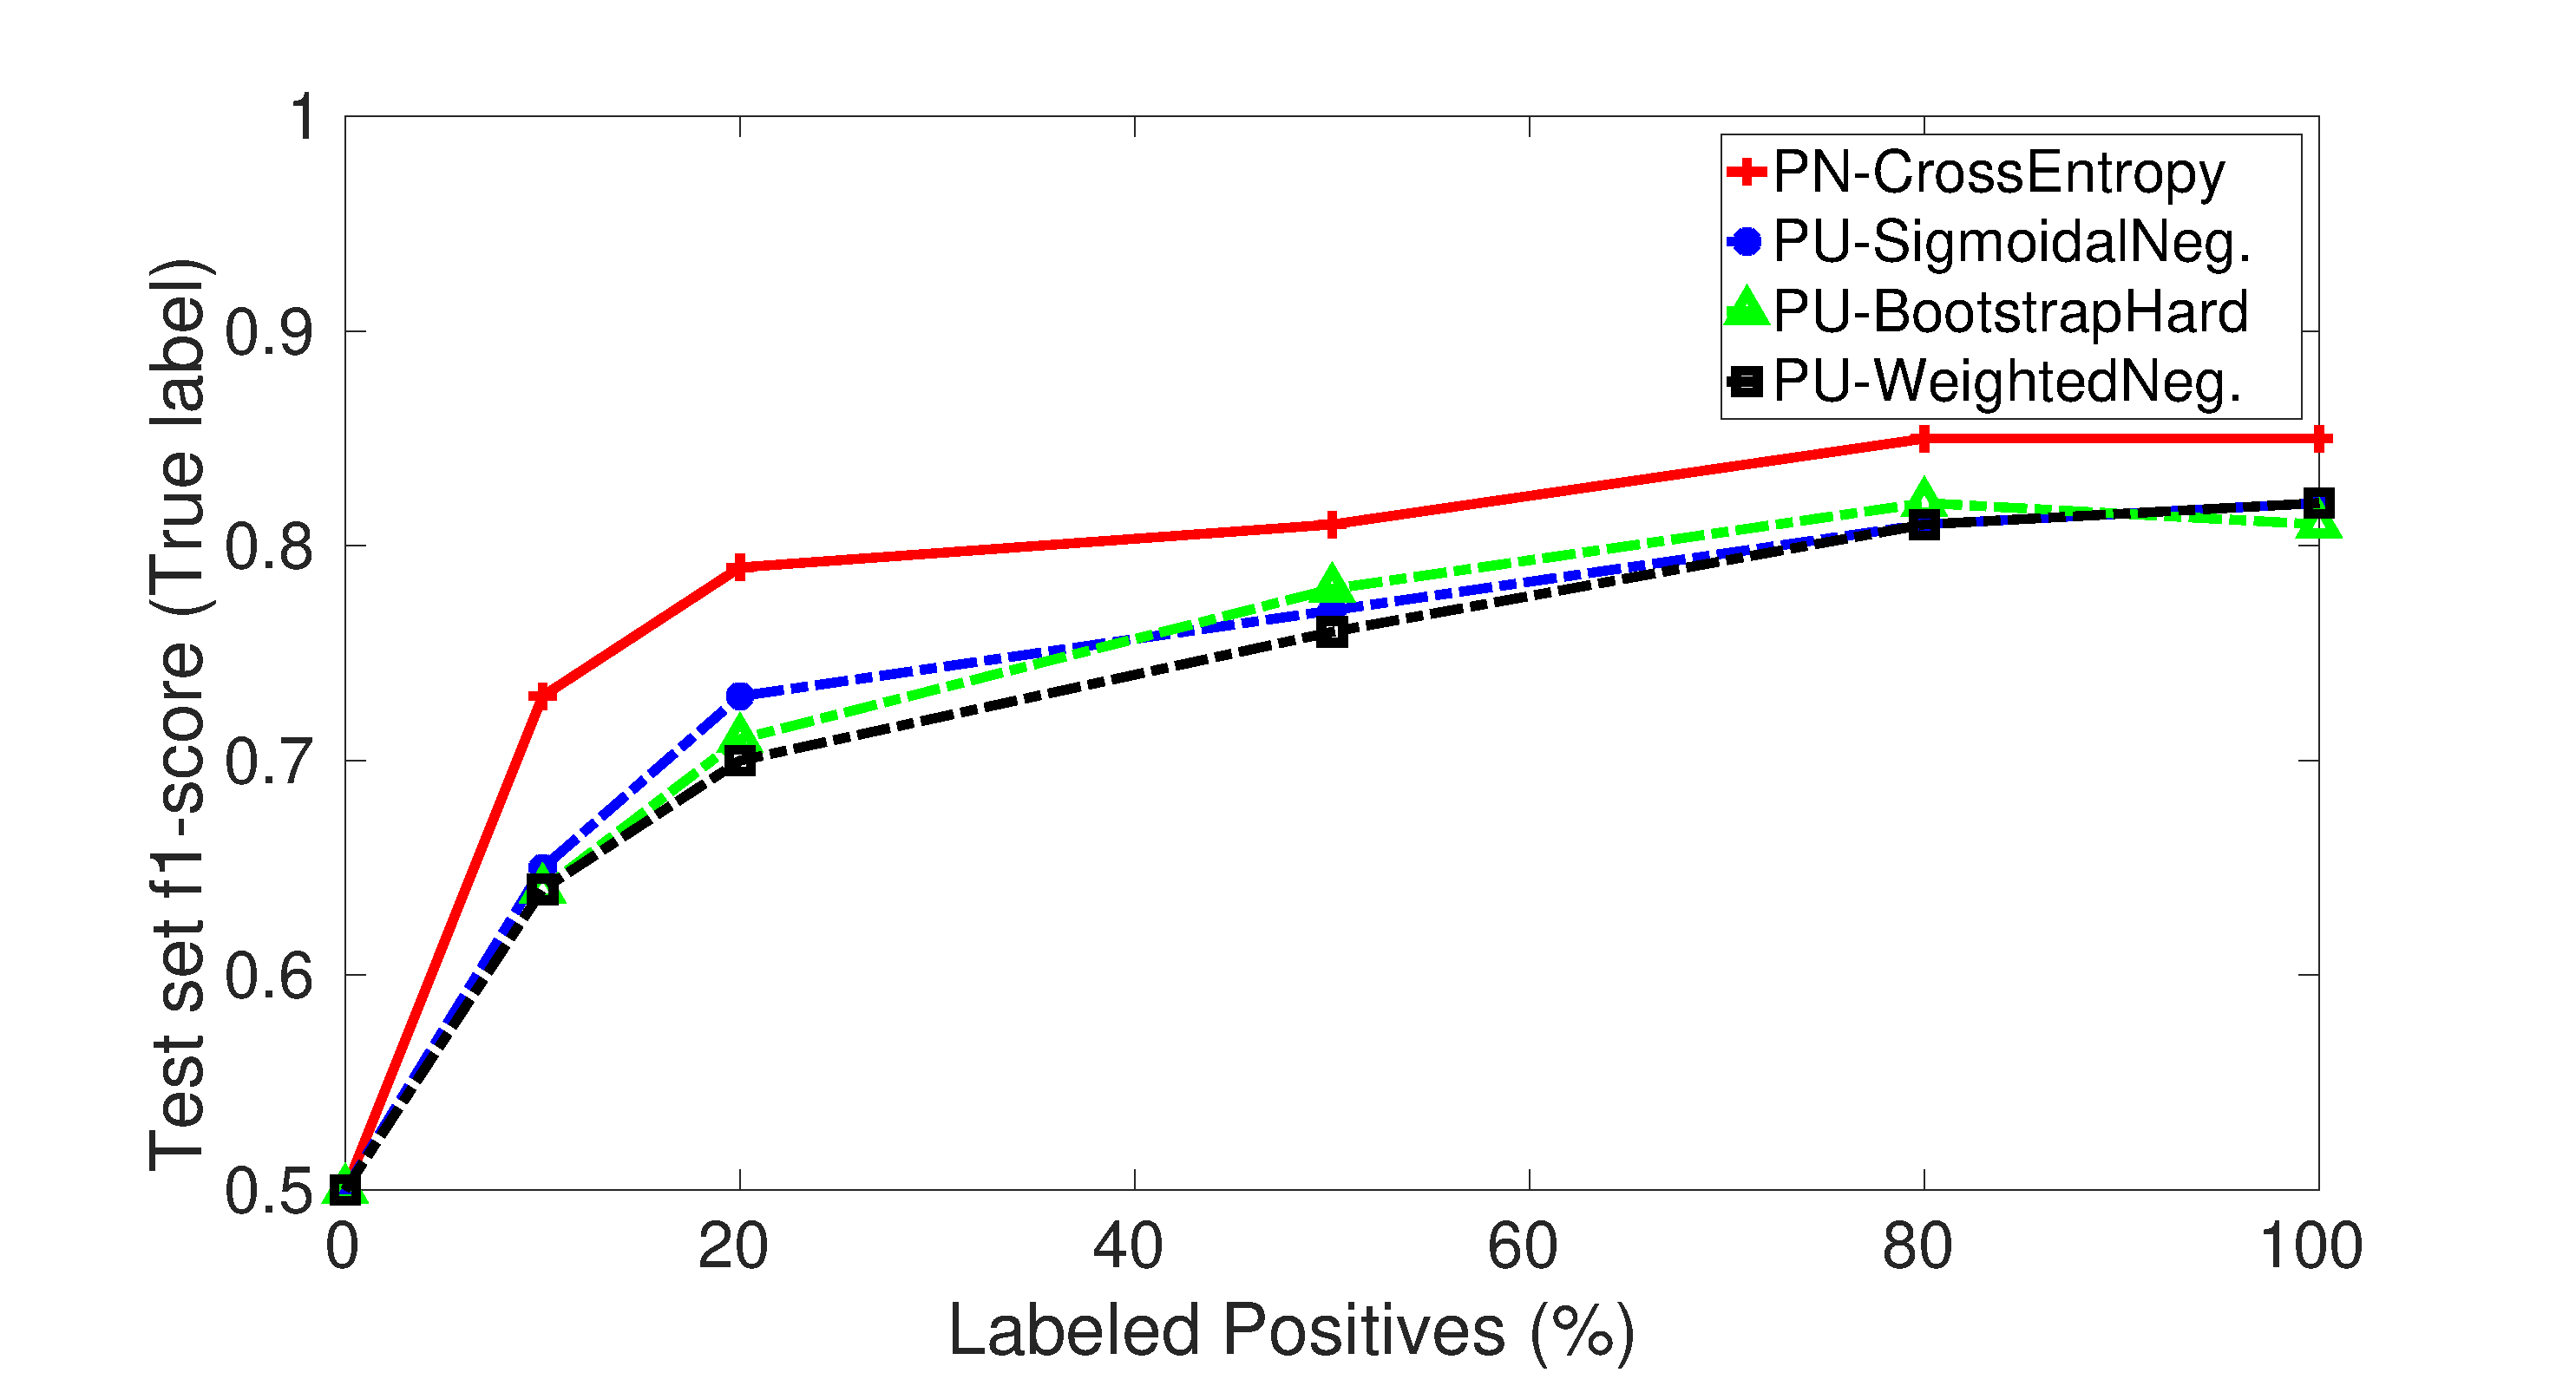
\includegraphics[width=\linewidth]{img/pu_vs_pn}
\caption{Varying percentage of labeled positive images. \textbf{P+N} represents training with percetage of images with reliable positive and negative labels and \textbf{P+U} stands for training with the positive (P) and unlabeled (U) sets.}
\label{fig:pct_annotating}
\end{figure}

%%%%%%%% Text Segmentation Pascal VOC2011
\paragraph{Pascal VOC2011 segmentation task}
In the segmentation setup, we used again the PASCAL VOC2011 dataset with extra segmentation\cite{hariharan2011semantic}.
We synthesized inexhaustive segmentations the same way as described in Section \ref{subsec:robustness}.
The same AlexNet-FCN model were trained together with the different loss functions for class 0 to predict binary segmentation, determining whether a pixel is correspondent to an object or not.
Only single-object images were used for training and testing in order to avoid the influence of two adjacent objects joining as one object because of  binary segmentation.
The same hyperparameters for optimization were used as in Section \ref{subsec:robustness}.
The trained models were evaluated with the test set of PASACAL VOC2011 segmentation dataset with binary segmentations.

\noindent
As shown in Table \ref{tab:pusegment}, the exponential unlabeled loss achieved the highest mean accuracy and a slightly lower overall accuracy.
In contrast to the improvement of mean accuracy, mean IU for models trained with either weighted unlabeled loss or exponential unlabeled loss did not show significant improvement to the normal cross entropy loss.


%%%%%%%% TABLE Segmentation Pascal VOC2011
\begin{table}[t]
\resizebox{\columnwidth}{!}{
\centering
\begin{tabular}{ll|llll}
Annotation  & Loss & overall acc. & mean acc. & f.w. IU & mean IU \\
\hline
% Complete            & CrossEnt.U       &  0.88 & 0.60 & 0.48 & 0.80 \\
% 50\%Unsegmented     & CrossEnt.U       &  0.83 & 0.31 & 0.27 & 0.70 \\
% 50\%Unsegmented     & WeightedU        &  0.83 & 0.34 & 0.29 & 0.70 \\
% 50\%Unsegmented     & ExponentialU     &  0.83 & 0.34 & 0.29 & 0.70 \\
Complete       & CrossEnt.U       &  0.90 & 0.85 & 0.82 & 0.75 \\
50\%Unseg.     & CrossEnt.U       &  0.85 & 0.68 & 0.73 & 0.60 \\
50\%Unseg.     & WeightedU        &  0.84 & 0.71 & 0.73 & \textbf{0.62} \\
50\%Unseg.     & ExponentialU     &  0.83 & \textbf{0.75} & 0.72 & \textbf{0.62} \\
\end{tabular}
}
\caption{
Best binary segmentation performance achieved on the test set of PASCAL VOC2011 segmentation dataset in the presence of inexhaustive segmentation.
Class weight 0.7:1.75 was used to balance the sample frequency differences of the two classes and negative loss were further weighted by a factor of 0.5 for weighted unlabeled loss.
Mean accuracy is equivalent to mean recall over classes.
Mean IU is the average intersection over union ratio (IU) over two classes and f.w. IU is the frequency weighted average of IU over the two classes.
Experiments were repeated twice and standard deviations were approximately 0.01.
}
\label{tab:pusegment}
\end{table}


%%%%%%%% Figure Segmentation Pascawl VOC2011
\noindent
Selective predictions for models trained with exponential unlabeled (ExpU.) loss and normal cross entropy (CrossEnt.) loss were presented in Figure \ref{fig:pusegment}.
For these two example images, the model trained with cross entropy loss failed to segment objects from images whereas exponential unlabeled loss segmented on the position of the objects though with coarse outlines.
The third column shows predictions given by model trained with complete training segmentation, and it did not give more accurate outlines.
The coarse results were mainly due to the limited compacity of AlexNet model.

\begin{figure}
\centering
  \begin{minipage}{\columnwidth}\footnotesize
  \centering
  \subsubfloat{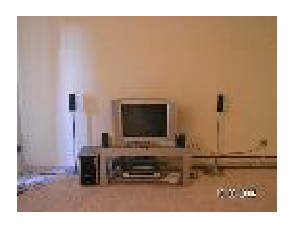
\includegraphics[width=0.19\columnwidth]{img/2007_002132}}{Raw}
  \subsubfloat{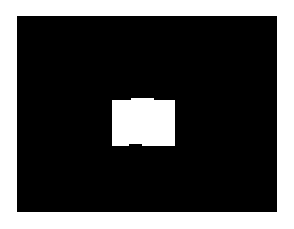
\includegraphics[width=0.19\columnwidth]{img/2007_002132_label}}{Label}
  \subsubfloat{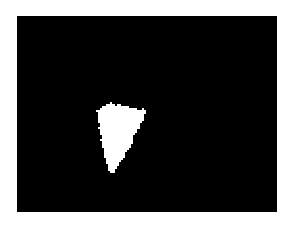
\includegraphics[width=0.19\columnwidth]{img/2007_002132_up_pred}}{Complete}
  \subsubfloat{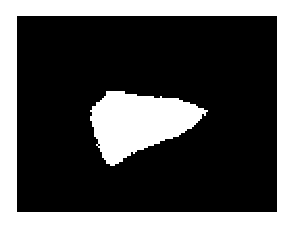
\includegraphics[width=0.19\columnwidth]{img/2007_002132_exp_pred}}{ExpU.}
  \subsubfloat{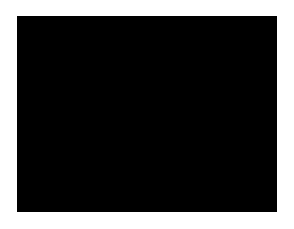
\includegraphics[width=0.19\columnwidth]{img/2007_002132_low_pred}}{CrossEnt.}
  \subsubfloat{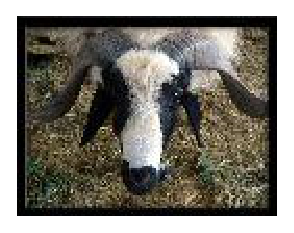
\includegraphics[width=0.19\columnwidth]{img/2007_002618}}{Raw}%
  \subsubfloat{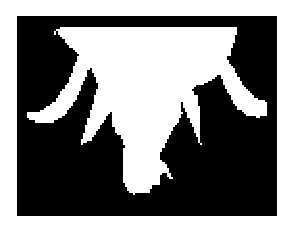
\includegraphics[width=0.19\columnwidth]{img/2007_002618_label}}{Label}
  \subsubfloat{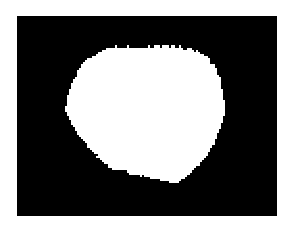
\includegraphics[width=0.19\columnwidth]{img/2007_002618_up_pred}}{Complete}
  \subsubfloat{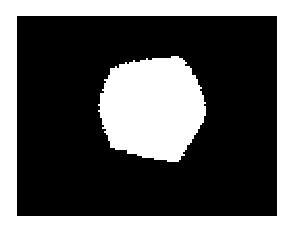
\includegraphics[width=0.19\columnwidth]{img/2007_002618_exp_pred}}{ExpU.}
  \subsubfloat{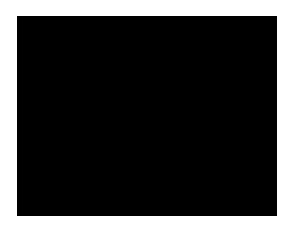
\includegraphics[width=0.19\columnwidth]{img/2007_002618_low_pred}}{CrossEnt.}
  \end{minipage}
\caption{Selective predictions for models in Table \ref{tab:pusegment}.}
\label{fig:pusegment}
\end{figure}


%%%%%%%% Text Fine-tuning performance with exponential loss
\noindent \textit{Exponential loss help improve fine-tuning performance}
Additionally,
